\subsubsection{Rotation-numbers in the \Glsentrylong{pal} Structures}

\todo{replace cycles with correct notation for cycles in full model}

Next, we will take a look at the rotation-numbers in the Farey-trees of the \gls{pal} structures.
Note that we don't have two branches in the archetypal model, instead we have four.
This means, that the definition \Cref{def:rotation.numbers} does not work for our case.
Instead, we define rotation-tuples.
\Cref{fig:add.prop.rot.num.tree} shows as Farey-tree with rotation-tuples.

\begin{definition}[Rotation Tuples]
	The rotation tuple of a cycle with the symbolic sequence $\phi$ in the archetypal model is defined as the following.
	\begin{align}
		\rho(\phi)
		= \left(\rho_\A(\phi), \rho_\B(\phi), \rho_\C(\phi), \rho_\D(\phi)\right)
		= \left(\dfrac{|\phi|_\A}{|\phi|}, \dfrac{|\phi|_\B}{|\phi|}, \dfrac{|\phi|_\C}{|\phi|}, \dfrac{|\phi|_\D}{|\phi|}\right)
	\end{align}
	Where $|\phi|_\A$ is the number of symbols $\A$ in the sequence.
	Analogous for the symbols $\B$, $\C$, and $\D$.
\end{definition}

\begin{figure}
	\centering
	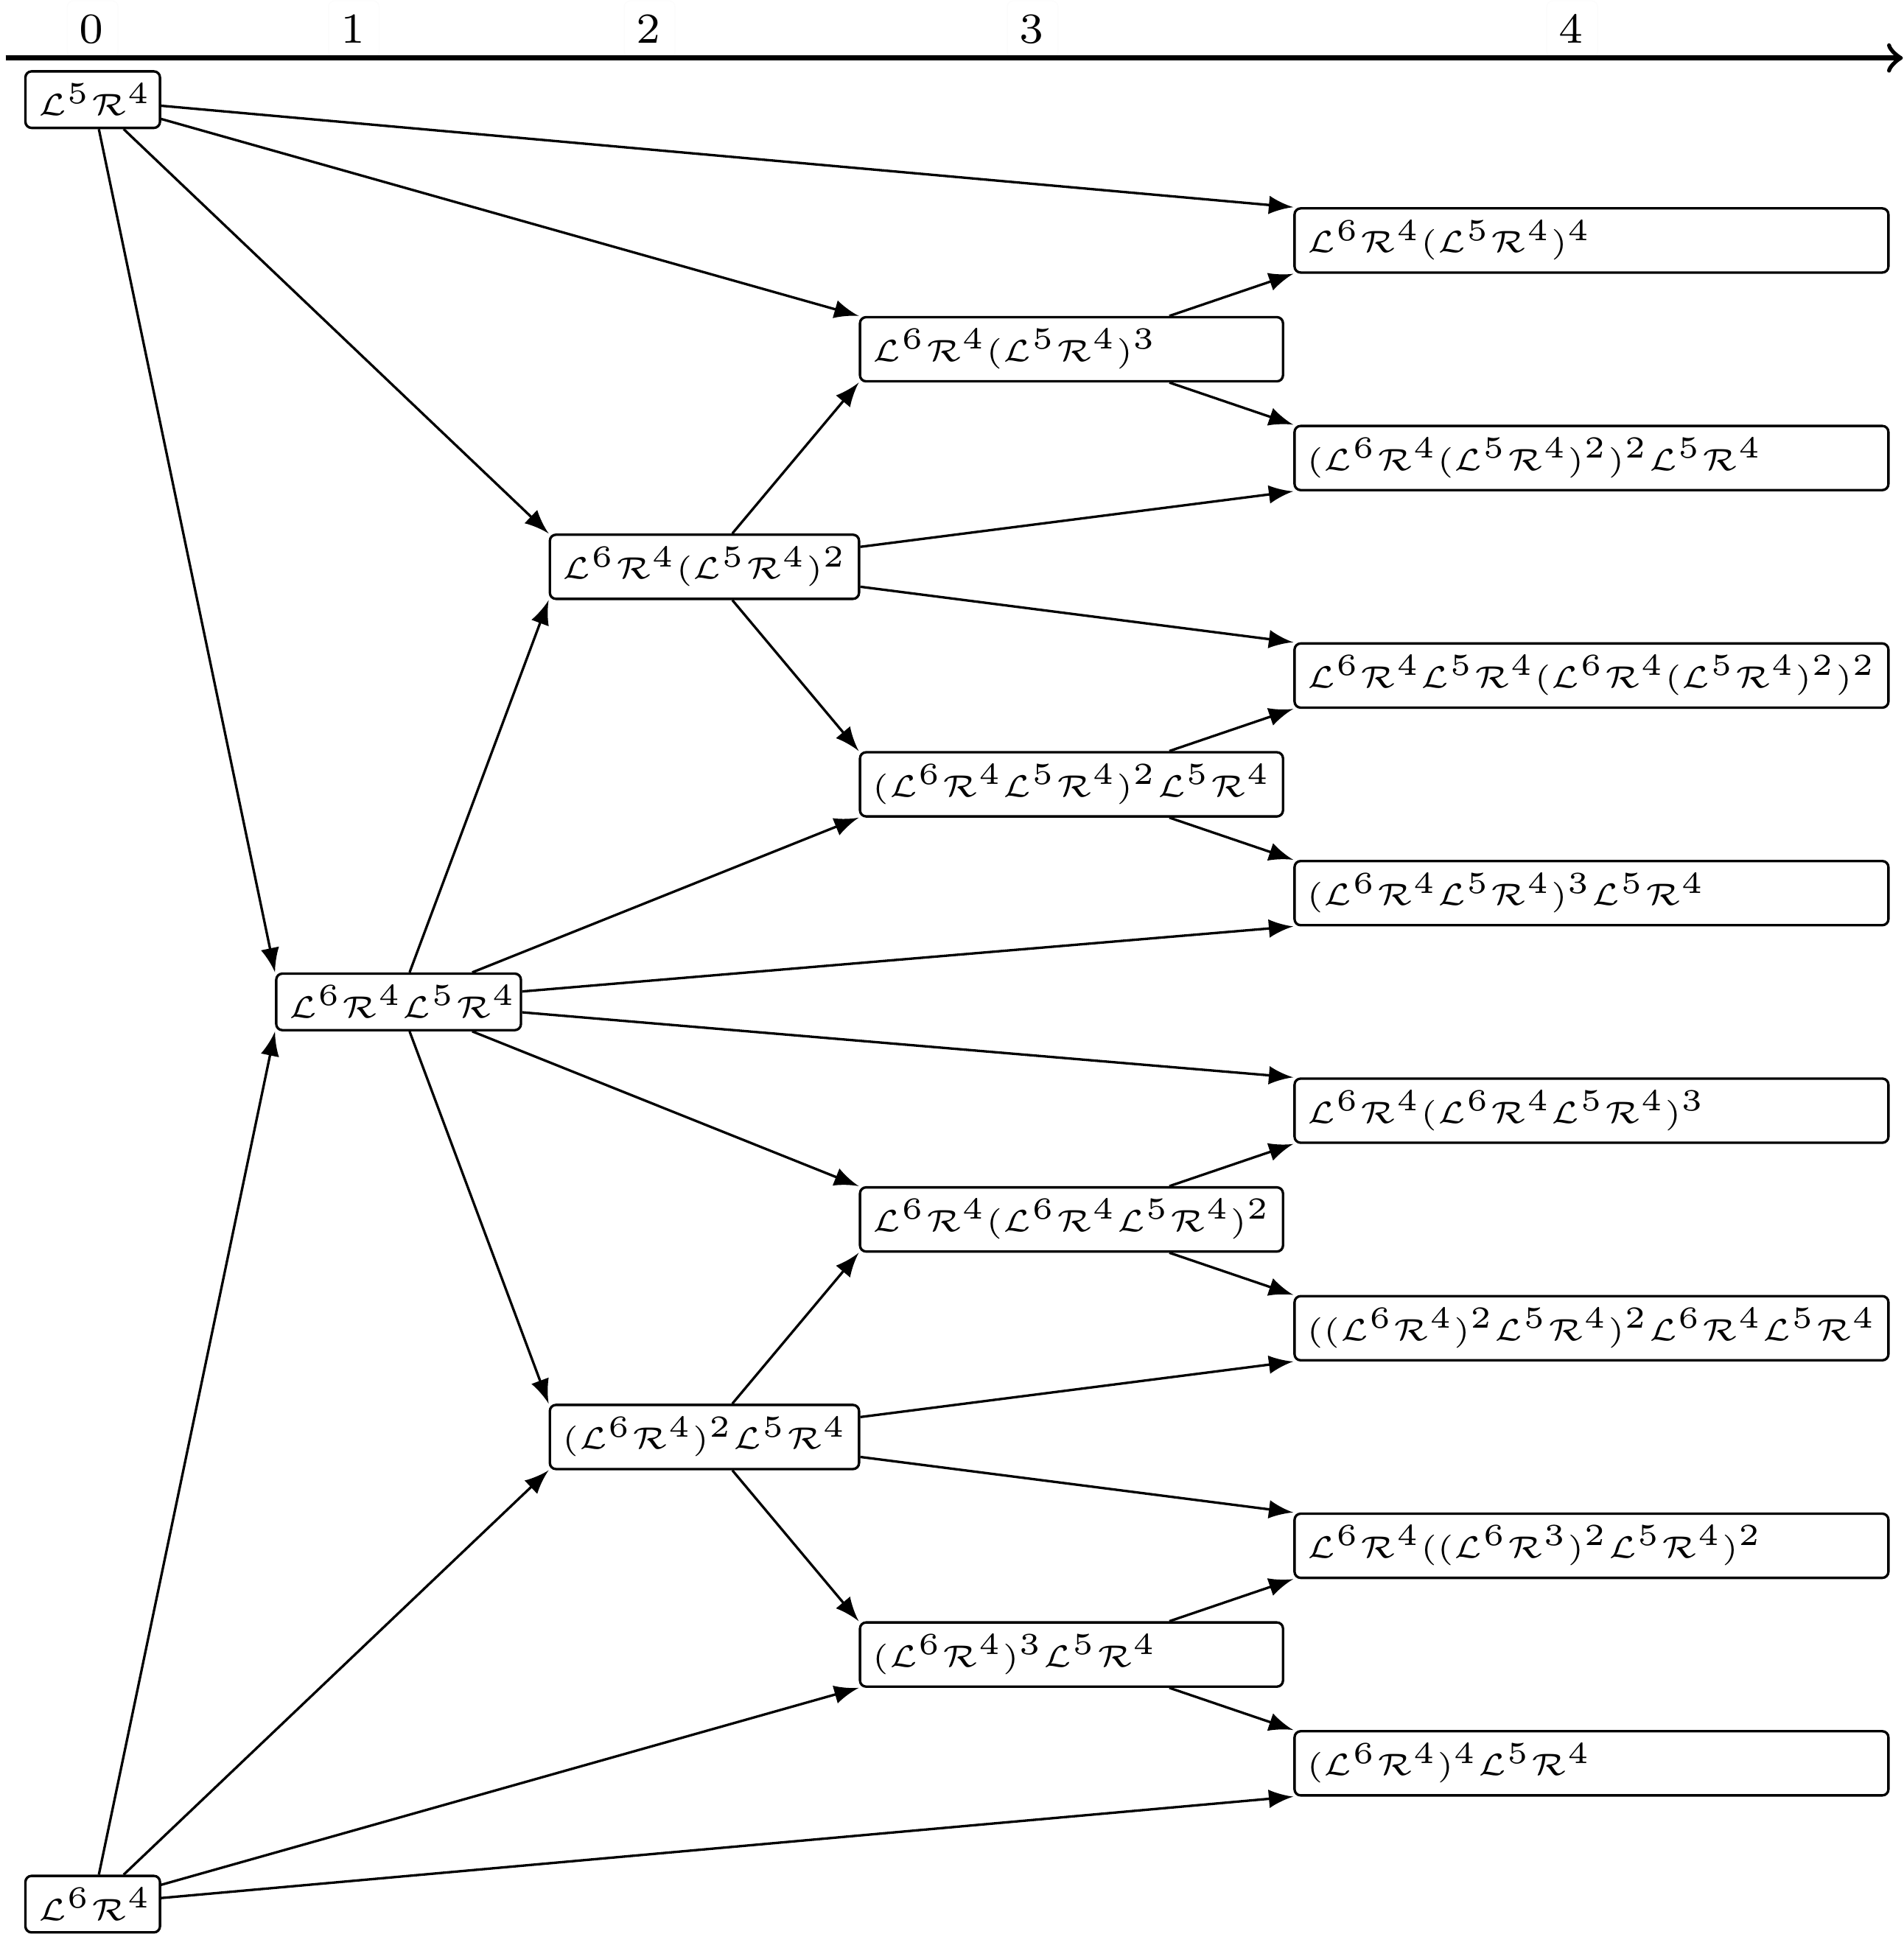
\includegraphics[width=.8 \textwidth]{FareyTrees/Minrep_Adding1_Full_RotNum/adding.png}
	\caption{Farey tree with rotation numbers}
	\label{fig:add.prop.rot.num.tree}
\end{figure}


\begin{theorem}[Rotation Tuples of Child Nodes I]
	The child node of two nodes that are both associated with a single cycle each with the symbolic sequences $\phi$ and $\psi$ is associated with the following period.
	We will call the symbolic sequences of the two cycles associated with the child node $\pi^a$ and $\pi^b$ in the following.
	\begin{align*}
		|\pi^a| = |\pi^b| & = \dfrac{|\sigma| + |\varrho|}{2} = |\pi|
	\end{align*}
	And its rotation tuples are the following.
	\begin{align*}
		\rho_\A(\pi^a) & = \dfrac{\left|\phi_1 \dots \phi_{\frac{n+1}{2}}\right|_\A + \left|\psi_{\frac{m+3}{2}} \dots \psi_m\right|_\A}{|\pi|} \\
		\rho_\B(\pi^a) & = \dfrac{\left|\phi_1 \dots \phi_{\frac{n+1}{2}}\right|_\B + \left|\psi_{\frac{m+3}{2}} \dots \psi_m\right|_\B}{|\pi|} \\
		\rho_\C(\pi^a) & = \dfrac{\left|\phi_1 \dots \phi_{\frac{n-1}{2}}\right|_\C + \left|\psi_{\frac{m+1}{2}} \dots \psi_m\right|_\C}{|\pi|} \\
		\rho_\D(\pi^a) & = \dfrac{\left|\phi_1 \dots \phi_{\frac{n-1}{2}}\right|_\D + \left|\psi_{\frac{m+1}{2}} \dots \psi_m\right|_\D}{|\pi|} \\
		\rho_\A(\pi^b) & = \dfrac{\left|\psi_1 \dots \psi_{\frac{m+1}{2}}\right|_\A + \left|\phi_{\frac{n+3}{2}} \dots \phi_n\right|_\A}{|\pi|} \\
		\rho_\B(\pi^b) & = \dfrac{\left|\psi_1 \dots \psi_{\frac{m+1}{2}}\right|_\B + \left|\phi_{\frac{n+3}{2}} \dots \phi_n\right|_\B}{|\pi|} \\
		\rho_\C(\pi^b) & = \dfrac{\left|\psi_1 \dots \psi_{\frac{m-1}{2}}\right|_\C + \left|\phi_{\frac{n+1}{2}} \dots \phi_n\right|_\C}{|\pi|} \\
		\rho_\D(\pi^b) & = \dfrac{\left|\psi_1 \dots \psi_{\frac{m-1}{2}}\right|_\D + \left|\phi_{\frac{n+1}{2}} \dots \phi_n\right|_\D}{|\pi|}
	\end{align*}
\end{theorem}

\begin{proof} \phantom{x} \\
	Let $\sigma = \sigma_1\sigma_2 \dots \sigma_i$ with odd $i$, $\varrho = \varrho_1\varrho_2 \dots \varrho_j$ with odd $j$, $T(\sigma) = \phi$, and $T(\varrho) = \psi$.
	The child of both nodes in the halved archetypal model is associated with the symbolic sequence $\sigma\varrho = \sigma_1 \dots \sigma_i \varrho_1 \dots \varrho_j$.
	This manifests as two coexisting cycles in the archetypal model with the symbolic sequences $\pi^a$ and $\pi^b$ following the rules in \Cref{theorem:child.symbolic.1}.


	We start by proving the period of the cycles with symbolic sequences $\pi^a$ and $\pi^b$.
	\begin{align*}
		|\pi^a| & = |T(\sigma\varrho)|                                                               \\
		        & = |T(\sigma_1 \dots \sigma_i \varrho_1 \dots \varrho_j)|                           \\
		        & = |t(\sigma_1\sigma_2) \dots t(\sigma_i\varrho_1) \dots t(\varrho_{j-1}\varrho_j)| \\
		        & = |\sigma_1\sigma_2 \dots \sigma_i \varrho_1 \dots \varrho_{j-1}\varrho_j|         \\
		        & = |\sigma\varrho| = \frac{|\phi|}{2} + \frac{|\psi|}{2}
	\end{align*}
	Note that the last step takes advantage of the fact about the periods of cycles in the archetypal model described in \Cref{theorem:period.pal}.
	The proof for $\pi^b$ is similar and has the same result.
	\begin{align*}
		|\pi^b| & = |T(s_2(\sigma\varrho))|                                                                              \\
		        & = |T(\sigma_2 \dots \sigma_i \varrho_1 \dots \varrho_j \sigma_1)|                                      \\
		        & = |t(\sigma_2\sigma_3) \dots t(\sigma_{i-1}\sigma_i) t(\varrho_1\varrho_2) \dots t(\varrho_j\sigma_1)| \\
		        & = |\sigma_2\sigma_3 \dots \sigma_i \varrho_1 \dots \varrho_j \sigma_1|                                 \\
		        & = |\sigma_1\sigma_2 \dots \sigma_i \varrho_1 \dots \varrho_j|                                          \\
		        & = |\sigma\varrho| = \frac{|\phi|}{2} + \frac{|\psi|}{2}
	\end{align*}

	This gives us the denominators of all elements of both rotation tuples.
	For the numerators, we have to count the symbols in the symbolic sequences of the cycles associated with each child node.
	We start with $\pi^a$ and the symbol $\A$.
	\begin{align*}
		|\pi^a|_\A & = \left|\phi_1 \dots \phi_{\frac{n-1}{2}} \left[\phi_{\frac{n+1}{2}} \mid \psi_{\frac{m+1}{2}}\right] \psi_{\frac{m+3}{2}} \dots \psi_m\right|_\A                \\
		           & = |\phi_1|_\A + \dots + \left|\left[\phi_{\frac{n+1}{2}} \mid \psi_{\frac{n+1}{2}}\right]\right|_\A + \left|\psi_{\frac{m+3}{2}}\right|_\A + \dots + |\psi_m|_\A \\
		           & = |\phi_1|_\A + \dots + \left|\phi_{\frac{n+1}{2}}\right|_\A + \left|\psi_{\frac{m+3}{2}}\right|_\A + \dots + |\psi_m|_\A                                        \\
		           & = \left|\phi_1 \dots \phi_{\frac{n+1}{2}}\right|_\A + \left|\psi_{\frac{m+3}{2}} \dots \psi_m\right|_\A
	\end{align*}
	We can do the second to last step, since the symbol $\A$ is in the first 2-syllable of $\phi_{\frac{n+1}{2}}$.
	The same is true for the symbol $\B$ and the proof works exactly the same for $|\pi^a|\B$, so we will omit it here.
	For the symbols $\C$ and $\D$ the last step does not work, instead we have to choose $\psi_{\frac{n+1}{2}}$.
	We demonstrate it for $|\pi^a|_\C$, the proof for $|\pi^a|_\D$ works exactly the same.
	\begin{align*}
		|\pi^a|_\C & = \left|\phi_1 \dots \phi_{\frac{n-1}{2}} \left[\phi_{\frac{n+1}{2}} \mid \psi_{\frac{m+1}{2}}\right] \psi_{\frac{m+3}{2}} \dots \psi_m\right|_\C                \\
		           & = |\phi_1|_\C + \dots + \left|\left[\phi_{\frac{n+1}{2}} \mid \psi_{\frac{n+1}{2}}\right]\right|_\C + \left|\psi_{\frac{m+3}{2}}\right|_\C + \dots + |\psi_m|_\C \\
		           & = |\phi_1|_\C + \dots + \left|\psi_{\frac{n+1}{2}}\right|_\C + \left|\psi_{\frac{m+3}{2}}\right|_\C + \dots + |\psi_m|_\C                                        \\
		           & = \left|\phi_1 \dots \psi_{\frac{n+1}{2}}\right|_\C + \left|\psi_{\frac{m+3}{2}} \dots \psi_m\right|_\C
	\end{align*}

	Now we will take a look at the numerators of the elements in the rotation tuple of $\pi^b$.
	We start with the symbol $\A$.
	\begin{align*}
		|\pi^b|_\A & = \left|\phi_{\frac{n+3}{2}} \dots \phi_n \psi_1 \dots \psi_{\frac{m-1}{2}} \left[\psi_{\frac{m+1}{2}} \mid \phi_{\frac{n+1}{2}}\right]\right|_\A                                                       \\
		           & = \left|\phi_{\frac{n+3}{2}}\right|_\A + \dots + |\phi_n|_\A + |\psi_1|_\A + \dots + \left|\psi_{\frac{m-1}{2}}\right|_\A + \left|\left[\psi_{\frac{m+1}{2}} \mid \phi_{\frac{n+1}{2}}\right]\right|_\A \\
		           & = \left|\phi_{\frac{n+3}{2}}\right|_\A + \dots + |\phi_n|_\A + |\psi_1|_\A + \dots + \left|\psi_{\frac{m-1}{2}}\right|_\A + \left|\psi_{\frac{m+1}{2}}\right|_\A                                        \\
		           & = \left|\phi_{\frac{n+3}{2}} \dots \phi_n\right|_\A + \left|\psi_1 \dots \psi_{\frac{m-1}{2}}\right|_\A + \left|\psi_{\frac{m+1}{2}}\right|_\A
	\end{align*}
	Again, we can do the second to last step, since the symbol $\A$ is in the first 2-syllable of $\psi_{\frac{n+1}{2}}$.
	The same is true for the symbol $\B$ and the proof works exactly the same for $|\pi^b|\B$.
	We will omit it here.
	For the symbols $\C$ and $\D$ the last step does not work, instead we have to choose $\phi_{\frac{n+1}{2}}$.
	We demonstrate it for $|\pi^b|_\C$, the proof for $|\pi^b|_\D$ works exactly the same.
	\begin{align*}
		|\pi^b|_\C & = \left|\phi_{\frac{n+3}{2}} \dots \phi_n \psi_1 \dots \psi_{\frac{m-1}{2}} \left[\psi_{\frac{m+1}{2}} \mid \phi_{\frac{n+1}{2}}\right]\right|_\C                                                       \\
		           & = \left|\phi_{\frac{n+3}{2}}\right|_\C + \dots + |\phi_n|_\A + |\psi_1|_\C + \dots + \left|\psi_{\frac{m-1}{2}}\right|_\C + \left|\left[\psi_{\frac{m+1}{2}} \mid \phi_{\frac{n+1}{2}}\right]\right|_\C \\
		           & = \left|\phi_{\frac{n+3}{2}}\right|_\C + \dots + |\phi_n|_\C + |\psi_1|_\C + \dots + \left|\psi_{\frac{m-1}{2}}\right|_\C + \left|\psi_{\frac{m+1}{2}}\right|_\C                                        \\
		           & = \left|\phi_{\frac{n+3}{2}} \dots \phi_n\right|_\C + \left|\psi_1 \dots \psi_{\frac{m-1}{2}} \psi_{\frac{m+1}{2}}\right|_\C
	\end{align*}
	\hfill $\blacksquare$
\end{proof}

\begin{theorem}[Rotation Tuples of Child Nodes II]
	The child node of a node with a singular cycle $\phi$ and a node with two coexisting cycles $\psi^a$ and $\psi^b$ will have the following rotation-like numbers.
	We will call the cycle associated with the child node $\pi$ in the following.
	\begin{align*}
		\rho_\A(\pi) & =
		\rho_\A(\phi) \oplus \rho_\A(\psi^a) \oplus \rho_A(\psi^b) \\
		\rho_\B(\pi) & =
		\rho_\B(\phi) \oplus \rho_\B(\psi^a) \oplus \rho_B(\psi^b) \\
		\rho_\C(\pi) & =
		\rho_\C(\phi) \oplus \rho_\C(\psi^a) \oplus \rho_C(\psi^b) \\
		\rho_\D(\pi) & =
		\rho_\D(\phi) \oplus \rho_\D(\psi^a) \oplus \rho_D(\psi^b)
	\end{align*}
\end{theorem}

\begin{proof} \phantom{x} \\
	We prove this again in two parts.
	First, we prove that the denominator of each element of the rotation tuples add up.
	\begin{align*}
		|\pi| & = \left|
		\phi_1 \dots \phi_{\frac{n-1}{2}} \left[\phi_{\frac{n+1}{2}} \mid \psi^b_m\right]
		\psi^b_1 \dots \psi^b_{m-1} \left[\psi^b_m \mid \phi_{\frac{n+1}{2}}\right]
		\phi_{\frac{n+3}{2}} \dots \phi_n \psi^a
		\right|                                                       \\
		      & = \left|
		\phi_1 \dots \phi_{\frac{n-1}{2}} \left[\phi_{\frac{n+1}{2}} \mid \phi_{\frac{n+1}{2}}\right]
		\phi_{\frac{n+3}{2}} \dots \phi_n
		\psi^b_1 \dots \psi^b_{m-1} \left[\psi^b_m \mid \psi^b_m\right]
		\psi^a
		\right|                                                       \\
		      & = |\phi \psi^b \psi^a| = |\phi| + |\psi^a| + |\psi^b|
	\end{align*}
	Note that the first step is achieved by simply reordering some 4-syllables and two 2-syllables in the symbolic sequences.
	This does not change the period.
	It does also not change the number of symbols, since we only swapped the second 2-syllable of $\left[\phi_{\frac{n+1}{2}} \mid \psi^b_m\right]$ and $\left[\psi^b_m \mid \phi_{\frac{n+1}{2}}\right]$.
	Therefore, the proof for works the same for the number of any symbol.
	We will demonstrate this for the symbol $\A$.
	\begin{align*}
		|\pi|_\A & = \left|
		\phi_1 \dots \phi_{\frac{n-1}{2}} \left[\phi_{\frac{n+1}{2}} \mid \psi^b_m\right]
		\psi^b_1 \dots \psi^b_{m-1} \left[\psi^b_m \mid \phi_{\frac{n+1}{2}}\right]
		\phi_{\frac{n+3}{2}} \dots \phi_n \psi^a
		\right|_\A                                                                   \\
		         & = \left|
		\phi_1 \dots \phi_{\frac{n-1}{2}} \left[\phi_{\frac{n+1}{2}} \mid \phi_{\frac{n+1}{2}}\right]
		\phi_{\frac{n+3}{2}} \dots \phi_n
		\psi^b_1 \dots \psi^b_{m-1} \left[\psi^b_m \mid \psi^b_m\right]
		\psi^a
		\right|_\A                                                                   \\
		         & = |\phi \psi^b \psi^a|_\A = |\phi|_\A + |\psi^a|_\A + |\psi^b|_\A
	\end{align*}
	Therefore the numerators of each element in the rotation tuples add up too.

	One might criticize that we only proved it for the case where the left parent node is associated with a single cycle.
	In that case
	\begin{align*}
		\pi = \phi_1 \dots \phi_{\frac{n-1}{2}} \left[\phi_{\frac{n+1}{2}} \mid \psi^b_m\right] \psi^b_1 \dots \psi^b_{m-1} \left[\psi^b_m \mid \phi_{\frac{n+1}{2}}\right] \phi_{\frac{n+3}{2}} \dots \phi_n \psi^a
	\end{align*}
	If the right parent node is associated with a single cycle, then
	\begin{align*}
		\pi = \psi^a \phi_1 \dots \phi_{\frac{n-1}{2}} \left[\phi_{\frac{n+1}{2}} \mid \psi^b_m\right] \psi^b_1 \dots \psi^b_{m-1} \left[\psi^b_m \mid \phi_{\frac{n+1}{2}}\right] \phi_{\frac{n+3}{2}} \dots \phi_n
	\end{align*}
	The only difference in both cases is that the symbols of $\psi^a$ are at the end in the first case and in the beginning in the second case.
	Therefore, the proof works also in this case.
	\hfill $\blacksquare$
\end{proof}

As mentioned before, the next case does not appear in the \gls{pal} structures we investigate.
But we will include it here again for completeness.

\begin{theorem}
	The child node of two nodes that are associated with two coexisting cycles each with symbolic sequences $\phi^a, \phi^b, \psi^a,$ and $\psi^b$ is associated with two coexisting cycles.
	We will call the two cycles associated with the child node $\pi^a$ and $\pi^b$ in the following.
	Their rotation tuples are $\rho(\pi^a) = (\rho_\A(\pi^a), \rho_\B(\pi^a), \rho_\C(\pi^a), \rho_\D(\pi^a))$ and $\rho(\pi^b) = (\rho_\A(\pi^b), \rho_\B(\pi^b), \rho_\C(\pi^b), \rho_\D(\pi^b))$ where the elements are defined as follows.
	\begin{subequations}
		\begin{align}
			\rho_\A(\pi^a) & = \rho_\A(\phi^a) \oplus \rho_\A(\psi^a) \\
			\rho_\B(\pi^a) & = \rho_\A(\phi^a) \oplus \rho_\A(\psi^a) \\
			\rho_\C(\pi^a) & = \rho_\A(\phi^a) \oplus \rho_\A(\psi^a) \\
			\rho_\D(\pi^a) & = \rho_\A(\phi^a) \oplus \rho_\A(\psi^a)
		\end{align}
	\end{subequations}
	And for the cycle with the symbolic sequence $\pi^b$.
	\begin{subequations}
		\begin{align}
			\rho_\A(\pi^b) & = \rho_\A(\phi^b) \oplus \rho_\A(\psi^b) \\
			\rho_\B(\pi^b) & = \rho_\A(\phi^b) \oplus \rho_\A(\psi^b) \\
			\rho_\C(\pi^b) & = \rho_\A(\phi^b) \oplus \rho_\A(\psi^b) \\
			\rho_\D(\pi^b) & = \rho_\A(\phi^b) \oplus \rho_\A(\psi^b)
		\end{align}
	\end{subequations}
\end{theorem}

\begin{proof} \phantom{x} \\
	We start with the cycle with symbolic sequence $\pi^a$.
	Again, we first prove that the denominators, i.e. the periods, add up.
	\begin{align*}
		|\pi^a| = |\phi^a\psi^a| = |\phi^a| + |\psi^a|
	\end{align*}
	This is straightforward and can be done for each symbol exactly like this.
	We will demonstrate it for the symbol $\A$.
	\begin{align*}
		|\pi^a|_\A = |\phi^a\psi^a|_\A = |\phi^a|_\A + |\psi^a|_\A
	\end{align*}
	Therefore, the numerators also add up.

	Now we prove the same thing for the cycle with symbolic sequence $\pi^b$.
	\begin{align*}
		|\pi^b| & = \left|\phi^b_1 \dots \phi^b_{n-1} \left[\phi^b_n \mid \psi^b_m\right] \psi^b_1 \dots \psi^b_{m-1} \left[\psi^b_m \mid \phi^b_n\right]\right| \\
		        & = \left|\phi^b_1 \dots \phi^b_{n-1} \left[\phi^b_n \mid \phi^b_n\right] \psi^b_1 \dots \psi^b_{m-1} \left[\psi^b_m \mid \psi^b_m\right]\right| \\
		        & = |\phi^b \psi^b| = |\phi^b| + |\psi^b|
	\end{align*}
	Here we simply swapped the second 2-syllables of $\left[\phi^b_n \mid \psi^b_m\right]$ and $\left[\psi^b_m \mid \phi^b_n\right]$.
	This does not change the period.
	It also does not change the number of any symbol.
	Therefore, we can use the same proof for any symbol.
	We demonstrate it for the symbol $\A$ in the following.
	\begin{align*}
		|\pi^b|_\A & = \left|\phi^b_1 \dots \phi^b_{n-1} \left[\phi^b_n \mid \psi^b_m\right] \psi^b_1 \dots \psi^b_{m-1} \left[\psi^b_m \mid \phi^b_n\right]\right|_\A \\
		           & = \left|\phi^b_1 \dots \phi^b_{n-1} \left[\phi^b_n \mid \phi^b_n\right] \psi^b_1 \dots \psi^b_{m-1} \left[\psi^b_m \mid \psi^b_m\right]\right|_\A \\
		           & = |\phi^b \psi^b|_\A = |\phi^b|_\A + |\psi^b|_\A
	\end{align*}
	Therefore, the numerators also add up here.
	\hfill $\blacksquare$
\end{proof}

In the usual case with two symbols, the rotation numbers are monotone.
In our case, this is not true when considering the rotation tuples element-wise.
We can see a counter example in \Cref{fig:add.prop.rot.num.tree}.
$\dfrac{6}{19} > \dfrac{6}{20}$ and $\dfrac{6}{19} > \dfrac{5}{18}$.
But when considering the farey sum of the rotation-like numbers of coexisting cycles, the monotony holds.

\begin{theorem}{Monotony of Rotation-like Numbers in the Full Model}
	The rotation-like numbers for one symbol are monotone in the farey tree of a period-adding structure in the full model, when considering the farey sum of the rotation-like numbers of coexisting cycles.
	\todo{sentences too long and complicated in enumeration}
	\begin{enumerate}
		\item The rotation-like numbers that correspond to the cycle of a child node of a parent node with a singular cycle and a parent node of two coexisting cycles, is in between the corresponding rotation-like number of the parent node with a singular cycle and the corresponding sum of rotation-like numbers of the parent node with two coexisting cycles.
		      \begin{align*}
			           & \rho_X(\sigma) < \rho_X(\pi) < \rho_X(\varrho^a) \oplus \rho_X(\varrho^b) \\
			      \lor & \rho_X(\sigma) > \rho_X(\pi) > \rho_X(\varrho^a) \oplus \rho_X(\varrho^b)
		      \end{align*}
		\item The farey sum of the rotation-like numbers that correspond to each coexisting cycle of a child node of two nodes with a singular cycle each, is in between the corresponding rotation-like numbers of the parent nodes.
		      \begin{align*}
			           & \rho_X(\sigma) < \rho_X(\pi^a) \oplus \rho_X(\pi^b) < \rho_X(\varrho) \\
			      \lor & \rho_X(\sigma) > \rho_X(\pi^a) \oplus \rho_X(\pi^b) > \rho_X(\varrho)
		      \end{align*}
	\end{enumerate}
\end{theorem}

\begin{proof}
	\todo{prove}
\end{proof}

\todo{rotation numbers in the sense of poincare follow monotony directly, but coexisting cycles have same rotation numbers}

rotation number of coexisting cycles = rotation number of cycle in halved model

rotation number of single cycle = 2 $\otimes$ rotation number of cycle in halved model
